\chapter{Kết quả thực nghiệm và Đánh giá}
\label{chap:c4}

Chương này trình bày toàn diện các kết quả thu được từ quá trình nghiên cứu và triển khai hệ thống. Nội dung được tổ chức thành ba phần chính: đầu tiên là mô tả ứng dụng demo thực tế đã được xây dựng; tiếp theo là các kết quả thực nghiệm chi tiết về khả năng sinh dữ liệu, trích xuất đặc trưng và học liên tục; cuối cùng là các phân tích so sánh định lượng để làm rõ hiệu quả của các cải tiến đề xuất so với các phương pháp cơ sở.

\section{Thiết lập thực nghiệm và Kịch bản đánh giá trôi dạt khái niệm}

Thực nghiệm được thiết lập nhằm đánh giá khả năng học trực tuyến và độ ổn định cấu trúc của thuật toán EAGNG trên dòng dữ liệu khuyết tật màn hình điện thoại. Toàn bộ kịch bản kiểm thử được xây dựng theo tiêu chuẩn kiểm tra công nghiệp, bảo đảm tính thống nhất về môi trường tính toán, phương pháp trích xuất đặc trưng và hệ thống chỉ số đo lường.

\subsection{Môi trường thực nghiệm và Cơ sở hạ tầng tính toán}
\label{subsec:moi_truong_thuc_nghiem}

Môi trường phần cứng tính toán đóng vai trò quyết định đến độ tin cậy của việc đo lường thời gian xử lý trực tuyến. Hệ thống thực nghiệm được triển khai trên máy tính cấu hình bao gồm vi xử lý Intel Core i5-13400F, bộ nhớ truy cập ngẫu nhiên 16 gigabyte và bộ xử lý đồ họa NVIDIA GeForce RTX 3060 dung lượng 12 gigabyte. Cơ sở hạ tầng phần cứng này bảo đảm năng lực tính toán song song cho quá trình trích xuất đặc trưng và mô phỏng dòng dữ liệu thời gian thực.

Nền tảng phần mềm được xây dựng trên hệ điều hành Windows 11 nhằm duy trì tính đồng nhất trong quá trình thu thập dữ liệu. Môi trường tính toán sử dụng thư viện PyTorch phiên bản 2.13.0 kết hợp với thư viện Scikit-Learn phiên bản 1.9.0 cho các tác vụ xử lý ma trận và tính toán chỉ số phân cụm. Cấu hình chi tiết của cơ sở hạ tầng tính toán được tổng hợp trong Bảng \ref{tab:hardware_software_config}.

\begin{table}[htbp]
\centering
\caption{Thống kê thông số môi trường phần cứng và phần mềm thực nghiệm.}
\label{tab:hardware_software_config}
\begin{tabular}{|l|l|}
\hline
Thành phần hệ thống & Thông số kỹ thuật \\ \hline
Vi xử lý & Intel Core i5-13400F \\ \hline
Bộ nhớ ngẫu nhiên RAM & 16 GB DDR4 \\ \hline
Bộ xử lý đồ họa GPU & NVIDIA GeForce RTX 3060 12 GB \\ \hline
Hệ điều hành & Windows 11 \\ \hline
Môi trường phần mềm & PyTorch 2.13.0, Scikit-Learn 1.9.0 \\ \hline
\end{tabular}
\end{table}

Hệ thống chỉ số đánh giá được thiết lập bao quát cả ba khía cạnh bao gồm chất lượng phân cụm, độ ổn định cấu trúc tô-pô và hiệu năng thời gian thực. Chất lượng phân cụm trực tuyến được định lượng thông qua ba chỉ số độc lập là chỉ số Rand điều chỉnh, thông tin tương hỗ chuẩn hóa và độ tinh khiết phân cụm.

Chỉ số Rand điều chỉnh đo lường mức độ tương đồng giữa kết quả phân cụm thu được và nhãn thực tế của dữ liệu, loại bỏ yếu tố trùng khớp ngẫu nhiên \cite{hubert1985comparing}. Công thức \ref{eq:ari} biểu diễn phép tính chỉ số Rand điều chỉnh:
\begin{equation}
ARI = \frac{\sum_{ij} \binom{n_{ij}}{2} - \left[ \sum_i \binom{a_i}{2} \sum_j \binom{b_j}{2} \right] / \binom{n}{2}}{\frac{1}{2} \left[ \sum_i \binom{a_i}{2} + \sum_j \binom{b_j}{2} \right] - \left[ \sum_i \binom{a_i}{2} \sum_j \binom{b_j}{2} \right] / \binom{n}{2}}
\label{eq:ari}
\end{equation}
Trong Công thức \ref{eq:ari}, ký hiệu $n_{ij}$ đại diện cho số lượng mẫu dữ liệu thuộc cùng cụm thứ $i$ và nhãn thực tế thứ $j$, ký hiệu $a_i$ thể hiện tổng số mẫu trong cụm $i$, ký hiệu $b_j$ đại diện cho tổng số mẫu mang nhãn $j$, và ký hiệu $n$ biểu thị tổng số mẫu dữ liệu trong dòng học tính đến thời điểm đánh giá.

Thông tin tương hỗ chuẩn hóa đánh giá lượng thông tin chia sẻ giữa cấu trúc phân cụm của mô hình và tập nhãn thực tế \cite{strehl2002cluster}. Giá trị thông tin tương hỗ chuẩn hóa được xác định theo Công thức \ref{eq:nmi}:
\begin{equation}
NMI(Y, C) = \frac{2 \cdot I(Y; C)}{H(Y) + H(C)}
\label{eq:nmi}
\end{equation}
Trong Công thức \ref{eq:nmi}, ký hiệu $I(Y; C)$ biểu thị lượng thông tin tương hỗ giữa tập nhãn thực tế $Y$ và tập cụm dự đoán $C$, trong khi ký hiệu $H(Y)$ và $H(C)$ đại diện cho độ dư thừa thông tin của tập nhãn thực tế và tập cụm thu được.

Độ tinh khiết phân cụm đo tỷ lệ phần trăm mẫu dữ liệu thuộc về lớp chiếm ưu thế nhất trong mỗi cụm thu được. Phép tính độ tinh khiết phân cụm được mô tả cụ thể trong Công thức \ref{eq:purity}:
\begin{equation}
Purity(Y, C) = \frac{1}{N} \sum_{k} \max_{j} |c_k \cap y_j|
\label{eq:purity}
\end{equation}
Trong Công thức \ref{eq:purity}, ký hiệu $N$ biểu thị tổng số mẫu dữ liệu xử lý, ký hiệu $c_k$ đại diện cho tập hợp các mẫu trong cụm thứ $k$, và ký hiệu $y_j$ đại diện cho tập hợp các mẫu có nhãn thực tế thứ $j$.

Mức độ ổn định cấu trúc tô-pô và khả năng kháng hiện tượng quên thảm họa được đo lường thông qua độ dời Euclid cấp hai trung bình của tập nút mạng qua các bước cập nhật dòng dữ liệu. Công thức \ref{eq:displacement} xác định độ dời của tập nút:
\begin{equation}
\Delta W = \frac{1}{|V_t|} \sum_{v \in V_t} \min_{u \in V_{t-1}} \|w_v^{(t)} - w_u^{(t-1)}\|_2
\label{eq:displacement}
\end{equation}
Trong Công thức \ref{eq:displacement}, ký hiệu $V_t$ đại diện cho tập hợp nút mạng tại bước thời gian $t$, ký hiệu $V_{t-1}$ đại diện cho tập hợp nút tại bước thời gian liền trước, ký hiệu $w_v^{(t)}$ biểu diễn véc-tơ trọng số của nút $v$ ở thời điểm $t$, và ký hiệu $w_u^{(t-1)}$ đại diện cho véc-tơ trọng số của nút $u$ ở thời điểm $t-1$.

Hiệu năng xử lý thời gian thực được định lượng thông qua chỉ số thời gian nhịp sản xuất trung bình trên mỗi mẫu dữ liệu. Phép tính thời gian nhịp sản xuất được thiết lập theo Công thức \ref{eq:takttime}:
\begin{equation}
Takt = \frac{T_{total}}{N_{samples}} \times 1000
\label{eq:takttime}
\end{equation}
Trong Công thức \ref{eq:takttime}, ký hiệu $T_{total}$ biểu thị tổng thời gian tích lũy dành cho quá trình cập nhật mô hình tính bằng giây, ký hiệu $N_{samples}$ đại diện cho số lượng mẫu đã xử lý, và giá trị $Takt$ trả về đơn vị mili-giây trên một mẫu.

\subsection{Cấu hình tham số thực nghiệm và thuật toán EAGNG}
\label{subsec:cau_hinh_tham_so}

Tập hợp các tham số thực nghiệm được thiết lập dựa trên kết quả thăm dò kiểm thử nhằm bảo đảm sự cân bằng giữa độ chính xác phân cụm và tốc độ xử lý thời gian thực. Các tham số hệ thống được phân chia thành ba nhóm chức năng chính bao gồm (i) nhóm tham số trích xuất đặc trưng và mô hình mã hóa tự động, (ii) nhóm tham số phát hiện bất thường ngoại tuyến, và (iii) nhóm tham số điều khiển tiến trình học động của thuật toán EAGNG.

Trong nhóm tham số trích xuất đặc trưng, ảnh bề mặt màn hình điện thoại được chuẩn hóa về kích thước $128 \times 128$ pixel. Cửa sổ tính toán bản đồ độ hỗn loạn cục bộ sử dụng kích thước $9 \times 9$ pixel với bán kính phần tử cấu trúc dạng đĩa bằng $4$ pixel. Mô hình mã hóa tự động nén đặc trưng bốn kênh về véc-tơ không gian ẩn có chiều $d = 64$. Quá trình huấn luyện mô hình mã hóa tự động được thực hiện với tốc độ học $\eta_{ae} = 10^{-3}$, kích thước lô dữ liệu $B = 64$ và số chu kỳ huấn luyện $E_{ae} = 10$.

Trong nhóm tham số phát hiện bất thường ngoại tuyến, mô hình biểu diễn phân phối sản phẩm đạt chuẩn được huấn luyện trong $10$ chu kỳ. Ngưỡng phân định sản phẩm bất thường dựa trên quy tắc ba lần độ lệch chuẩn với hệ số $\lambda_{\sigma} = 3{,}0$. Bộ nhớ đệm dành cho các mẫu dữ liệu khuyết tật phát sinh được thiết lập với dung lượng lưu trữ tối đa $S_{buf} = 1000$ mẫu.

Nhóm tham số điều khiển thuật toán EAGNG quy định các cơ chế cập nhật cấu trúc đồ thị và thích ứng trực tuyến. Đồ thị nơ-ron có giới hạn số lượng nút tối đa $N_{max} = 500$ nút và tuổi thọ tối đa của cạnh nối được thiết lập $a_{max} = 50$ bước thời gian. Chu kỳ sinh nút mới theo mức tích lũy sai số được định cấu hình sau mỗi $\lambda = 50$ bước lặp với hệ số chia sai số nút $\alpha = 0{,}5$ và hệ số suy giảm sai số toàn cục $\beta = 0{,}005$. Tốc độ học của nút chiến thắng và các nút lân cận lần lượt nhận giá trị $e_b = 0{,}1$ và $e_n = 0{,}001$.

Các cơ chế cải tiến chuyên biệt trong thuật toán EAGNG được điều khiển bởi các tham số không gian và thời gian. Bán kính quét vùng dữ liệu mới được thiết lập $R_{scan} = 10{,}0$, đòi hỏi tối thiểu $K_{spawn} = 10$ mẫu trong bộ đệm để kích hoạt tiến trình sinh nút và huấn luyện cục bộ trong $E_{local} = 20$ chu kỳ với chu kỳ chèn nút cục bộ $\lambda_{local} = 10$. Giới hạn mật độ cục bộ sử dụng khoảng cách tối thiểu $d_{min} = 5{,}0$ nhằm ngăn ngừa hiện tượng phân mảnh vùng biểu diễn. Hệ số suy giảm tốc độ học theo thời gian sử dụng hằng số thời gian $\tau = 1000$ bước lặp. Ngưỡng giao thoa diện tích giữa các cụm để quyết định nối cạnh được ấn định ở mức $T_{overlap} = 0{,}65$. Bảng \ref{tab:eagng_parameters} tổng hợp chi tiết toàn bộ tham số cài đặt trong thực nghiệm.

\begin{table}[htbp]
\centering
\caption{Tổng hợp giá trị cài đặt các tham số mô hình và thuật toán EAGNG trong thực nghiệm.}
\label{tab:eagng_parameters}

\renewcommand{\arraystretch}{1.15}
\setlength{\tabcolsep}{5pt}

\begin{tabularx}{\textwidth}{|l|c|c|X|}
\hline
Nhóm tham số & Ký hiệu & Giá trị & Ý nghĩa kỹ thuật \\ \hline

Trích xuất đặc trưng 
& - & $128 \times 128$ 
& Kích thước ảnh chuẩn hóa (pixel) \\ \hline

Cửa sổ entropy 
& - & $9 \times 9$ 
& Kích thước cửa sổ độ hỗn loạn (pixel) \\ \hline

Không gian ẩn 
& $d$ & $64$ 
& Số chiều véc-tơ biểu diễn ẩn \\ \hline

Tốc độ học mã hóa 
& $\eta_{ae}$ & $10^{-3}$ 
& Tốc độ học của mô hình Autoencoder \\ \hline

Lô huấn luyện 
& $B$ & $64$ 
& Kích thước lô dữ liệu Autoencoder \\ \hline

Ngưỡng bất thường 
& $\lambda_{\sigma}$ & $3{,}0$ 
& Hệ số ngưỡng phân định $3\sigma$ \\ \hline

Sức chứa bộ đệm 
& $S_{buf}$ & $1000$ 
& Số mẫu khuyết tật tối đa trong bộ đệm \\ \hline

Số nút tối đa 
& $N_{max}$ & $500$ 
& Giới hạn số nút tối đa của đồ thị \\ \hline

Tuổi thọ cạnh 
& $a_{max}$ & $50$ 
& Tuổi thọ tối đa của cạnh nối giữa các nút \\ \hline

Chu kỳ chèn nút 
& $\lambda$ & $50$ 
& Tần suất kiểm tra sinh nút theo sai số \\ \hline

Hệ số chia sai số 
& $\alpha$ & $0{,}5$ 
& Tỷ lệ phân chia sai số khi sinh nút mới \\ \hline

Suy giảm sai số 
& $\beta$ & $0{,}005$ 
& Tỷ lệ suy giảm sai số toàn cục \\ \hline

Tốc độ học nút chính 
& $e_b$ & $0{,}1$ 
& Tốc độ học của nút chiến thắng \\ \hline

Tốc độ học lân cận 
& $e_n$ & $0{,}001$ 
& Tốc độ học của các nút lân cận \\ \hline

Bán kính quét vùng 
& $R_{scan}$ & $10{,}0$ 
& Ngưỡng khoảng cách nhận diện vùng mới \\ \hline

Số mẫu sinh nút 
& $K_{spawn}$ & $10$ 
& Mẫu tối thiểu trong đệm để tạo nút mới \\ \hline

Khoảng cách mật độ 
& $d_{min}$ & $5{,}0$ 
& Ngưỡng khoảng cách mật độ tối thiểu \\ \hline

Hằng số thời gian 
& $\tau$ & $1000$ 
& Hằng số thời gian giảm tốc độ học \\ \hline

Ngưỡng giao thoa 
& $T_{overlap}$ & $0{,}65$ 
& Ngưỡng tỷ lệ giao thoa để nối cạnh \\ \hline

\end{tabularx}

\end{table}

\subsection{Kịch bản dòng dữ liệu khuyết tật liên tục}
\label{sec:4_1_2_data_stream_scenario}

Bộ dữ liệu thực nghiệm được xây dựng bao gồm $3000$ ảnh mô phỏng các dạng khuyết tật bề mặt màn hình điện thoại trong môi trường kiểm tra công nghiệp. Ảnh thu nhận ban đầu đạt độ phân giải $540 \times 1170$ pixel từ hệ thống máy ảnh công nghiệp chuyên dụng. Tất cả các ảnh sau đó được tiền xử lý và thu nhỏ về kích thước chuẩn $128 \times 128$ pixel để chuẩn hóa đầu vào cho quá trình trích xuất đặc trưng.

Mô hình trích xuất đặc trưng kết hợp mạng ResNet-50 \cite{he2016deep} với thuật toán tính độ hỗn loạn cục bộ nhằm tạo lập không gian đại diện bốn kênh bao gồm ba kênh màu và một kênh độ hỗn loạn. Không gian dữ liệu này tiếp tục được nén thông qua mô hình mạng mã hóa tự động để thu về véc-tơ đặc trưng ẩn có kích thước $64$ chiều. Quy trình trích xuất này hỗ trợ cô đọng thông tin cấu trúc hình học và gia tăng độ tương phản đối với các vùng khuyết tật có biên độ xám thấp.

Tập dữ liệu bao gồm năm dạng khuyết tật hình học riêng biệt với các mức độ cường độ hiển thị khác nhau. Hình \ref{fig:c4_pattern} minh họa năm loại khuyết tật bề mặt trong tập dữ liệu thực nghiệm, bao gồm: (i) dạng đường tròn tại vị trí a, (ii) dạng đường ngang tại vị trí b, (iii) dạng hình tam giác tại vị trí c, (iv) dạng đường dọc tại vị trí d, và (v) dạng hình chữ nhật tại vị trí e. Mỗi dạng khuyết tật lại được chia thành ba cấp độ cường độ hiển thị bao gồm cường độ mạnh, cường độ vừa, và cường độ yếu. Hình \ref{fig:c4_level_pattern} biểu diễn chi tiết ba mức độ cường độ của khuyết tật dạng đường tròn, trong đó vị trí a thể hiện mức độ mạnh với độ tương phản rõ nét, vị trí b thể hiện mức độ vừa, và vị trí c thể hiện mức độ yếu với biên giới mờ nhạt so với nền màn hình.

\begin{figure}[htbp]
    \centering
    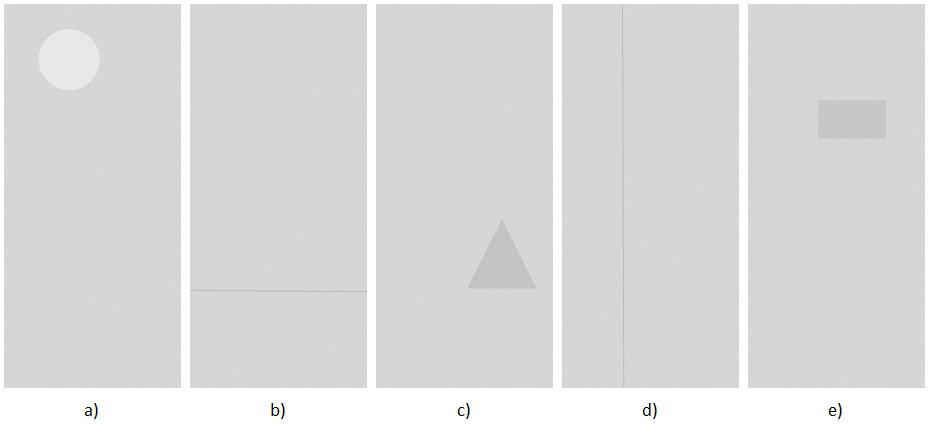
\includegraphics[width=0.85\linewidth]{figures/c4/c4_pattern.png}
    \caption{Năm dạng khuyết tật hình học bề mặt màn hình điện thoại trong tập dữ liệu thực nghiệm.}
    \label{fig:c4_pattern}
\end{figure}

\begin{figure}[htbp]
    \centering
    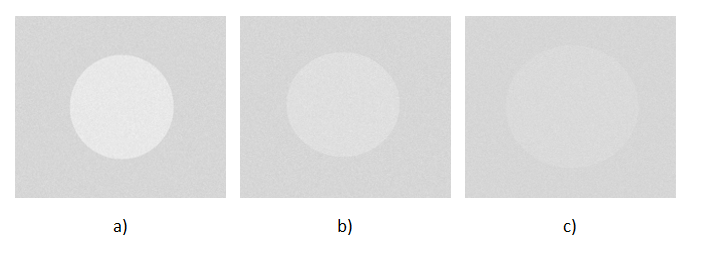
\includegraphics[width=0.75\linewidth]{figures/c4/c4_level_pattern.png}
    \caption{Ba cấp độ cường độ khuyết tật từ mạnh đến yếu đại diện cho dạng khuyết tật đường tròn.}
    \label{fig:c4_level_pattern}
\end{figure}

Dòng dữ liệu học trực tuyến được thiết lập dưới dạng chuỗi xuất hiện nối tiếp của năm loại khuyết tật qua năm giai đoạn liên tiếp nhằm tạo ra hiện tượng trôi dạt khái niệm đột ngột. Bảng \ref{tab:defect_summary} trình bày chi tiết sự phân bố mẫu, phạm vi chỉ số chuỗi dữ liệu và số lượng ảnh theo từng cấp độ cường độ khuyết tật. Mỗi loại khuyết tật đóng góp $600$ mẫu dữ liệu liên tục, trong đó mỗi cấp độ cường độ khuyết tật chiếm $200$ mẫu. Tại các mốc chuyển giao giữa các giai đoạn dữ liệu, sự thay đổi hoàn toàn của phân bố đặc trưng buộc thuật toán EAGNG phải thích ứng linh hoạt để tự động hình thành các nút biểu diễn mới mà không làm mất đi tri thức đã tích lũy từ các giai đoạn trước.

\begin{table}[htbp]
    \centering
    \caption{Thống kê chi tiết kịch bản phân bố dòng dữ liệu khuyết tật theo giai đoạn và cường độ.}
    \label{tab:defect_summary}
    \renewcommand{\arraystretch}{1.2}
    \begin{tabular}{|c|c|c|c|c|}
        \hline
        Giai đoạn & Loại khuyết tật & Cường độ khuyết tật & Phạm vi mẫu & Số lượng ảnh \\
        \hline
        1 & Đường tròn & Mạnh / Vừa / Yếu & 1--600 & 200 / 200 / 200 \\
        \hline
        2 & Đường ngang & Mạnh / Vừa / Yếu & 601--1200 & 200 / 200 / 200 \\
        \hline
        3 & Hình tam giác & Mạnh / Vừa / Yếu & 1201--1800 & 200 / 200 / 200 \\
        \hline
        4 & Đường dọc & Mạnh / Vừa / Yếu & 1801--2400 & 200 / 200 / 200 \\
        \hline
        5 & Hình chữ nhật & Mạnh / Vừa / Yếu & 2401--3000 & 200 / 200 / 200 \\
        \hline
    \end{tabular}
\end{table}
\section{Phân tích và Đánh giá Kết quả Thực nghiệm}
\label{sec:4_2_results}

Mục này trình bày kết quả thực nghiệm chi tiết đánh giá thuật toán Mạng Khí Nơ-ron Tăng trưởng Tích lũy Bằng chứng (Evidence-Accumulating Growing Neural Gas - EAGNG) trong bài toán phân loại lỗi tự động trên màn hình điện thoại. Việc đánh giá được thực hiện thông qua bốn nội dung chính bao gồm: (i) khả năng thích ứng với dịch chuyển khái niệm (Concept Drift), (ii) độ ổn định cấu trúc và hiện tượng quên thảm họa, (iii) thời gian xử lý và tốc độ thực thi, và (iv) hiệu quả phân cụm không gian hình học của không gian biểu diễn lỗi.

\subsection{Đánh giá khả năng thích ứng với dịch chuyển khái niệm}
\label{sec:4_2_1_concept_drift}

Khả năng thích ứng với dữ liệu chuỗi theo thời gian đóng vai trò quyết định đối với các mô hình học trực tuyến trong môi trường sản xuất công nghiệp. Thực nghiệm mô phỏng chuỗi dữ liệu gồm $3000$ mẫu với bốn điểm dịch chuyển khái niệm tại các thời điểm mẫu thứ $600$, $1200$, $1800$, và $2400$, tương ứng với sự xuất hiện của các dạng lỗi mới như đường kẻ ngang, hình tam giác, đường kẻ dọc, và hình chữ nhật. Kết quả đánh giá chỉ số điều chỉnh Rand (Adjusted Rand Index - ARI) thể hiện sự vượt trội của phương pháp đề xuất so với các thuật toán cơ sở.

\begin{figure}[htbp]
    \centering
    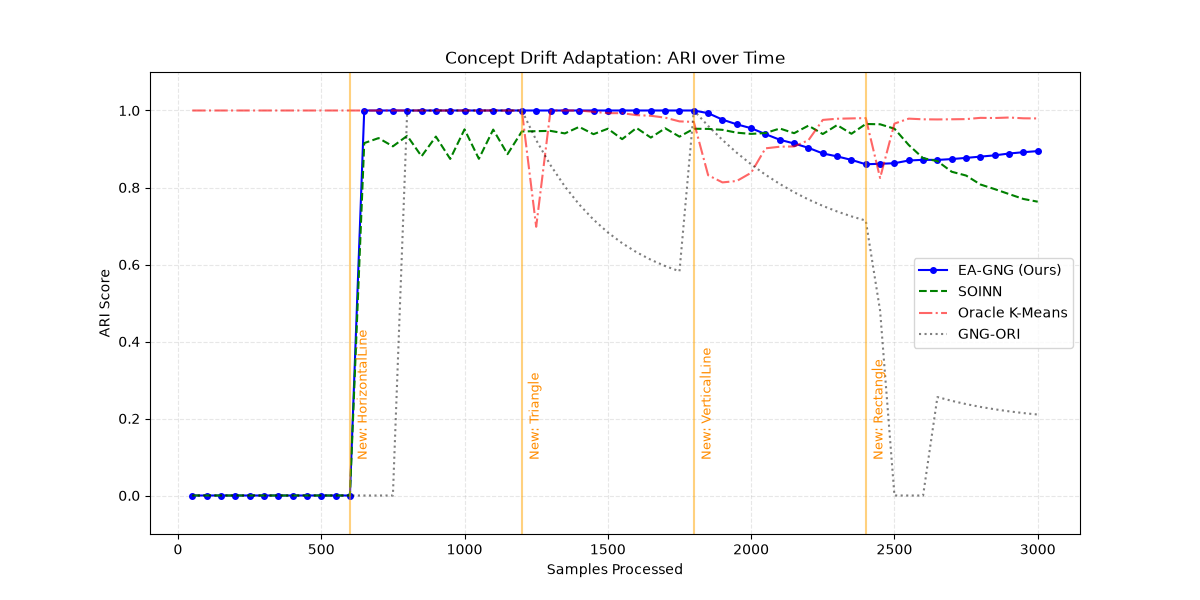
\includegraphics[width=0.9\linewidth]{figures/c4/c4_ARI.png}
    \caption{Sự biến thiên của chỉ số điều chỉnh Rand theo thời gian khi xuất hiện các dạng lỗi mới.}
    \caption*{Ghi chú: Đường nét liền màu xanh thể hiện phương pháp EAGNG, đường nét đứt màu xanh lá thể hiện SOINN, đường chấm chấm màu xám thể hiện GNG truyền thống, và đường gạch chấm màu đỏ thể hiện Oracle K-Means.}
    \label{fig:drift_ari}
\end{figure}

Như thể hiện trong Hình~\ref{fig:drift_ari}, chỉ số điều chỉnh Rand của thuật toán EAGNG nhanh chóng hội tụ về giá trị xấp xỉ $100\%$ ngay sau khi xuất hiện các dạng lỗi mới tại thời điểm $600$, $1200$, và $1800$. Đối với phương pháp GNG truyền thống \cite{fritzke1995growing}, chỉ số Rand suy giảm nghiêm trọng sau thời điểm $2400$, rơi xuống mức $21{,}0\%$ tại thời điểm $3000$ do hiện tượng nhiễu cấu trúc và không thể tách biệt các cụm lỗi trùng lặp. Phương pháp SOINN \cite{furao2006soinn} duy trì được tính ổn định tương đối nhưng chỉ đạt chỉ số Rand bằng $76{,}3\%$ tại bước $3000$, do cơ chế thiết lập ngưỡng bán kính cố định dẫn đến việc chia nhỏ các cụm lỗi tự nhiên.

\begin{figure}[htbp]
    \centering
    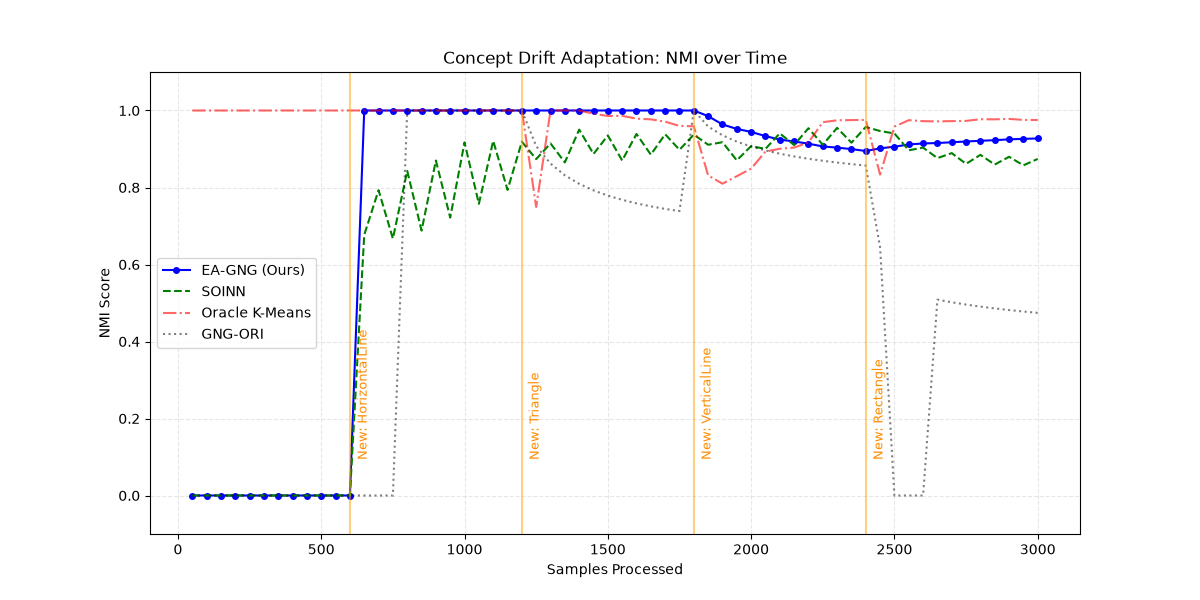
\includegraphics[width=0.9\linewidth]{figures/c4/c4_NMI.png}
    \caption{Sự biến thiên của chỉ số thông tin tương hỗ chuẩn hóa theo chuỗi thời gian xử lý mẫu.}
    \caption*{Ghi chú: Đánh giá khả năng bảo toàn thông tin phân cụm giữa kết quả của mô hình và nhãn thực tế.}
    \label{fig:drift_nmi}
\end{figure}

Chỉ số thông tin tương hỗ chuẩn hóa (Normalized Mutual Information - NMI) tiếp tục phản ánh khả năng phân tách cụm chính xác của mạng EAGNG trong suốt quá trình xử lý luồng dữ liệu. Hình~\ref{fig:drift_nmi} minh họa diễn biến chỉ số NMI giữa các phương pháp so sánh. Mạng EAGNG đạt chỉ số NMI duy trì ở mức $92{,}7\%$ tại mẫu thứ $3000$, trong khi GNG truyền thống suy giảm xuống $47{,}4\%$ và SOINN đạt $87{,}4\%$. Điều này chứng minh rằng cơ chế tích lũy bằng chứng giúp mô hình duy trì cấu trúc tô-pô biểu diễn chính xác thông tin phân bố của các lớp lỗi mà không bị ảnh hưởng bởi biến động nhiễu cục bộ.

\begin{figure}[htbp]
    \centering
    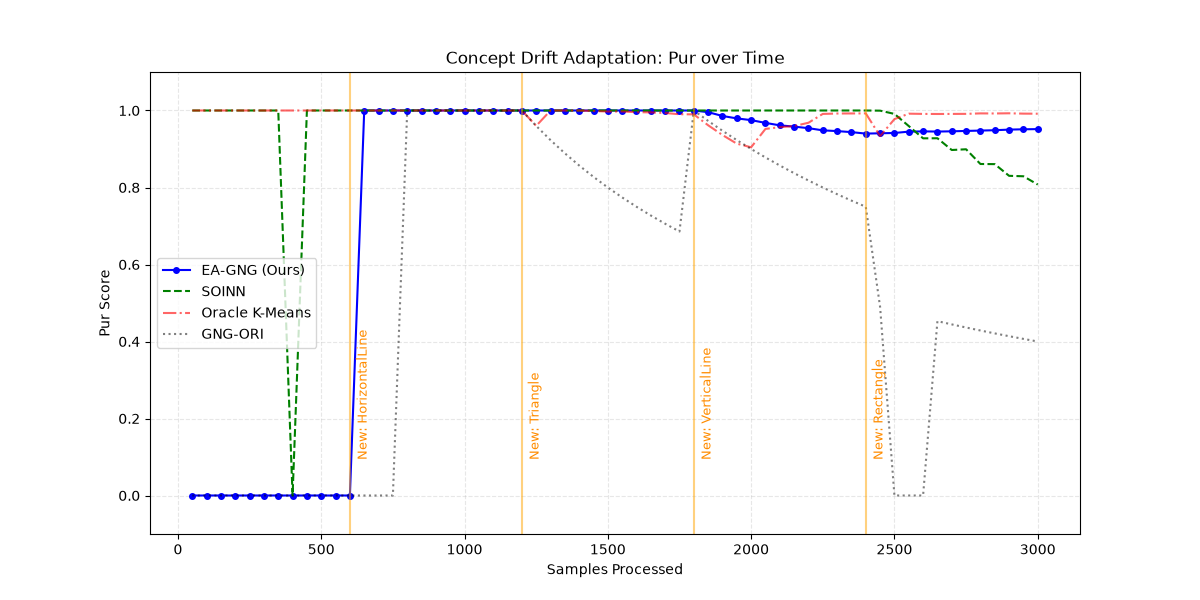
\includegraphics[width=0.9\linewidth]{figures/c4/c4_Pur.png}
    \caption{Chỉ số độ thuần khiết phân cụm của các thuật toán theo từng giai đoạn xuất hiện lỗi.}
    \caption*{Ghi chú: Mức độ thuần khiết phản ánh tỷ lệ mẫu thuộc lớp chiếm ưu thế trong từng cụm tô-pô.}
    \label{fig:drift_pur}
\end{figure}

Độ thuần khiết (Purity) của các cụm được khởi tạo bởi EAGNG thể hiện mức độ chính xác cao trong việc gom nhóm các mẫu lỗi có cùng bản chất kỹ thuật. Như được miêu tả ở Hình~\ref{fig:drift_pur}, độ thuần khiết của EAGNG đạt $95{,}2\%$ tại bước cuối cùng $3000$. Trái lại, phương pháp GNG truyền thống bị giảm độ thuần khiết xuống $40{,}0\%$ do các nơ-ron cũ bị kéo lệch khỏi tâm phân bố gốc khi dữ liệu mới xuất hiện. Sự duy trì độ thuần khiết cao của EAGNG khẳng định hiệu quả của cơ chế điều chỉnh độ linh hoạt dựa trên bằng chứng tích lũy.

\subsection{Phân tích độ ổn định cấu trúc và hiện tượng quên thảm họa}
\label{sec:4_2_2_stability}

Hiện tượng quên thảm họa là thách thức lớn đối với các mô hình học liên tục khi tiếp nhận các phân bố dữ liệu mới. Để đánh giá mức độ suy giảm tri thức cũ, khoảng cách dịch chuyển chuẩn L2 ($\Delta W$) của các nút đã tồn tại được đo đạc và theo dõi qua các bước cập nhật dữ liệu. 

\begin{figure}[htbp]
    \centering
    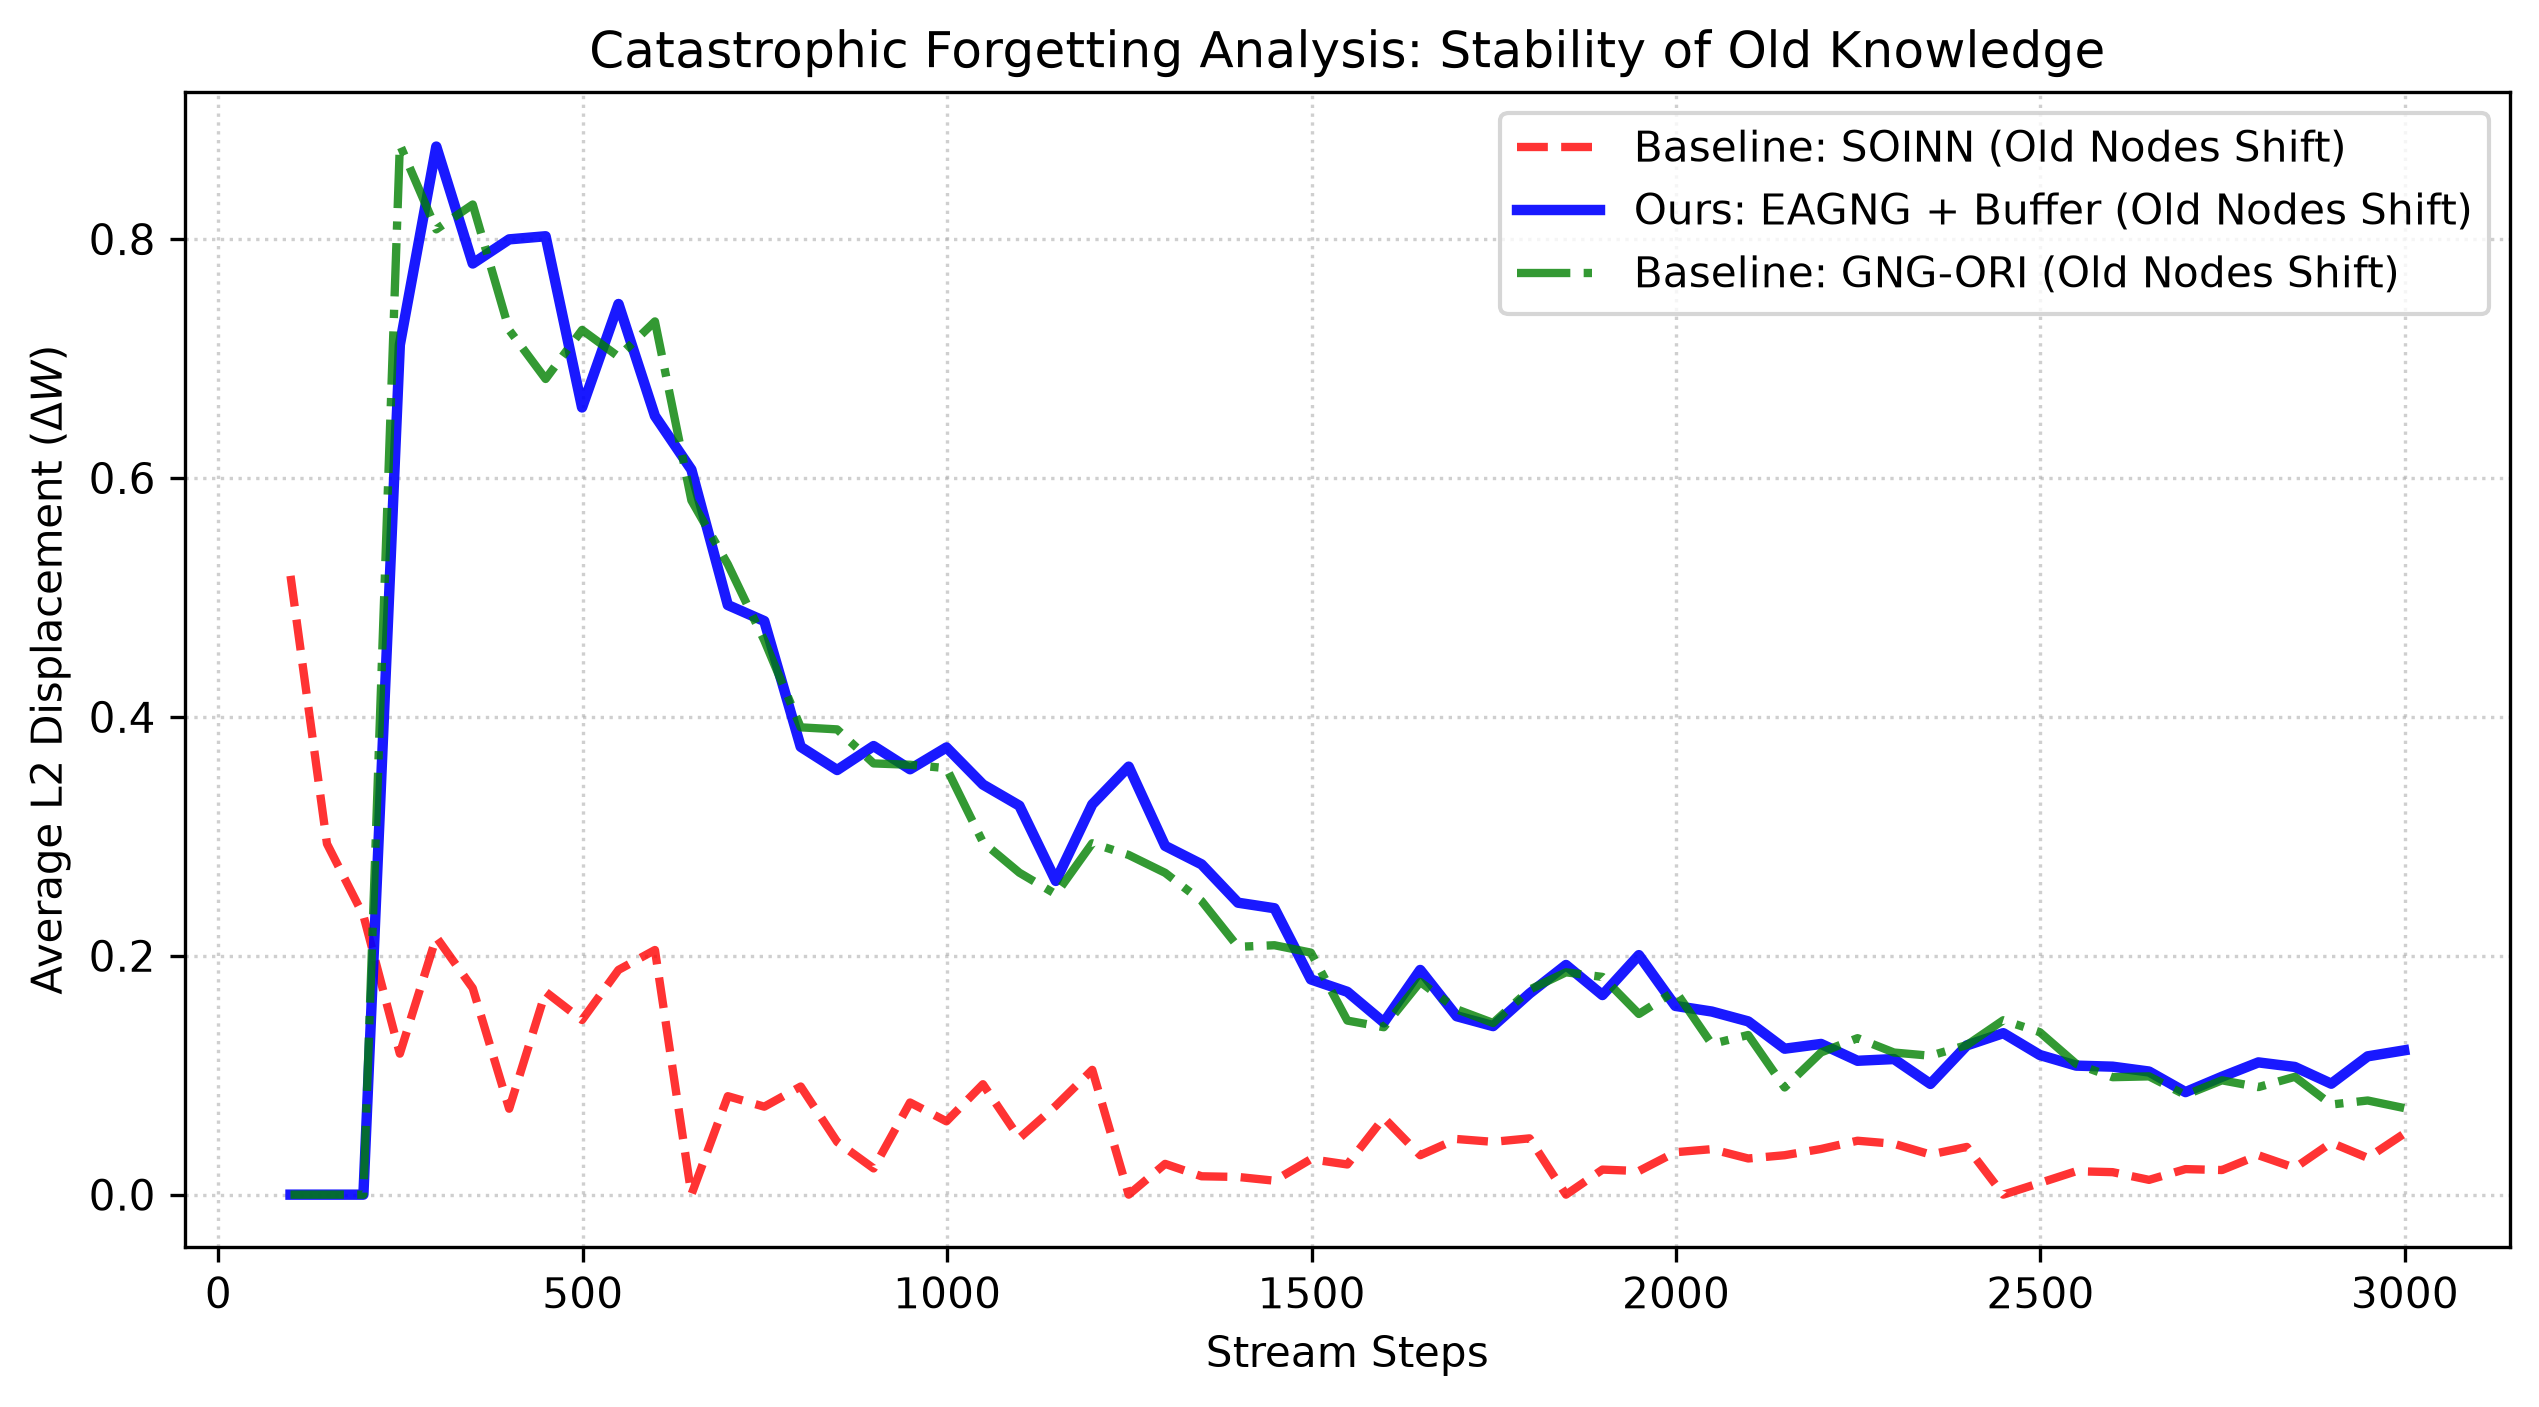
\includegraphics[width=0.85\linewidth]{figures/c4/c4_comparison.png}
    \caption{So sánh độ dịch chuyển trọng số nút cũ giữa các thuật toán theo chuỗi thời gian.}
    \caption*{Ghi chú: Giá trị độ dịch chuyển càng nhỏ thể hiện mức độ bảo toàn tri thức cũ càng cao.}
    \label{fig:stability_comp}
\end{figure}

Hình~\ref{fig:stability_comp} cho thấy mức độ dịch chuyển trọng số nút cũ của EAGNG kết hợp bộ đệm đạt giá trị xấp xỉ $0{,}10$ ở giai đoạn ổn định, thấp hơn đáng kể so với hiện tượng suy biến cấu trúc trong GNG truyền thống. Thuật toán SOINN duy trì mức dịch chuyển nhỏ nhưng đổi lại phải đánh đổi bằng việc khởi tạo quá nhiều nút không cần thiết. Phương pháp EAGNG đạt được sự cân bằng giữa việc tiếp thu tri thức mới và việc bảo toàn tri thức cũ nhờ vào bộ đệm tích lũy bằng chứng.

\begin{figure}[htbp]
    \centering
    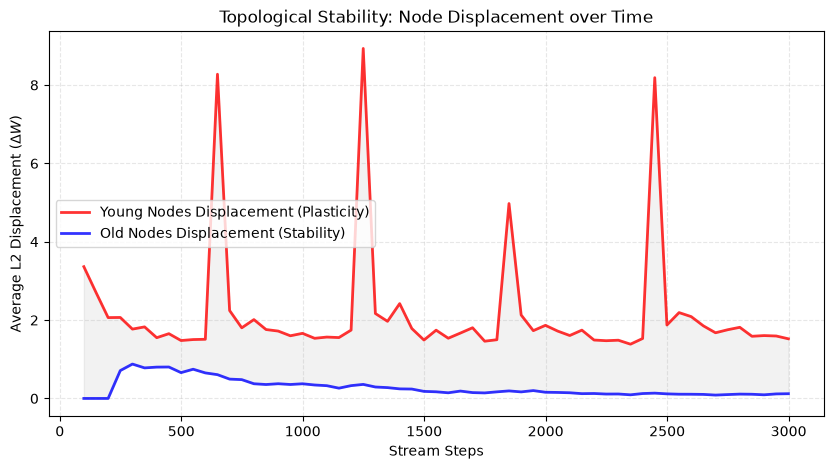
\includegraphics[width=0.85\linewidth]{figures/c4/c4_topological_stability.png}
    \caption{Phân tích khả năng thích ứng linh hoạt và độ ổn định tô-pô của mạng EAGNG.}
    \caption*{Ghi chú: Đường màu đỏ biểu diễn độ dịch chuyển của các nút mới (Plasticity), đường màu xanh biểu diễn độ dịch chuyển của các nút cũ (Stability).}
    \label{fig:topo_stability}
\end{figure}

Sự phân tách rõ rệt giữa tính linh hoạt (Plasticity) và tính ổn định (Stability) được thể hiện rõ ràng trong Công thức và cấu trúc tô-pô của EAGNG. Như miêu tả ở Hình~\ref{fig:topo_stability}, các nút mới (Young Nodes) đạt biên độ dịch chuyển trọng số lên tới $8{,}9$ tại các điểm xảy ra dịch chuyển khái niệm (bước $600$, $1200$, $1800$, $2400$), cho phép mạng thích ứng nhanh chóng với dạng lỗi mới. Trong khi đó, các nút cũ (Old Nodes) duy trì độ dịch chuyển trọng số luôn dưới $0{,}5$, đảm bảo các vùng không gian đại diện cho lỗi đã học không bị biến dạng.

\subsection{Đánh giá thời gian thực thi và tốc độ xử lý}
\label{sec:4_2_3_takt_time}

Tốc độ xử lý của thuật toán phân loại phải đáp ứng yêu cầu thời gian nhịp sản xuất (Takt Time) của dây chuyền kiểm tra màn hình điện thoại thực tế. Các chỉ số về thời gian tích lũy, thời gian xử lý trung bình trên mỗi mẫu (Takt Time), và tốc độ xử lý số mẫu trên giây (Throughput) được đo đạc trực tiếp trên cùng một cấu hình phần cứng.

\begin{figure}[htbp]
    \centering
    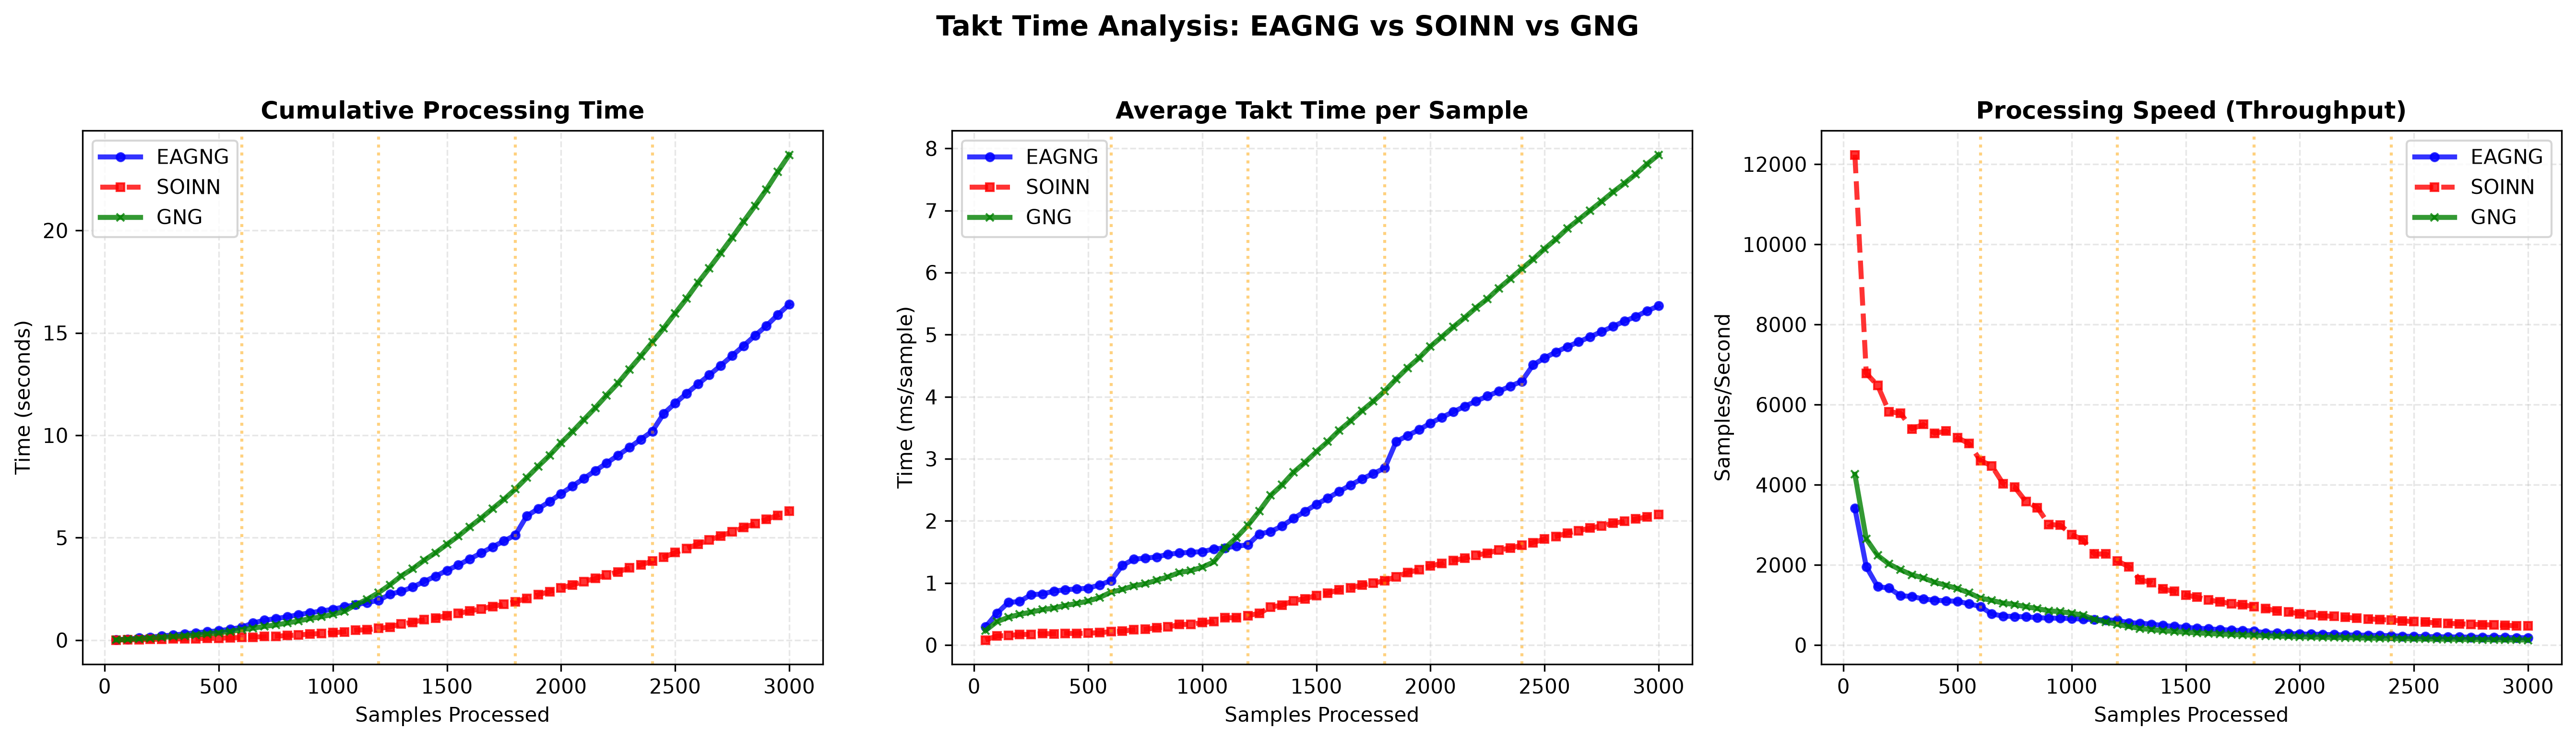
\includegraphics[width=0.98\linewidth]{figures/c4/c4_takt_time.png}
    \caption{Phân tích thời gian nhịp và tốc độ xử lý của EAGNG, SOINN và GNG.}
    \caption*{Ghi chú: Hình bên trái thể hiện thời gian xử lý tích lũy (giây), hình giữa thể hiện thời gian trung bình cho mỗi mẫu (mili-giây), hình bên phải thể hiện tốc độ xử lý (mẫu/giây).}
    \label{fig:takt_time}
\end{figure}

Như thể hiện trong Hình~\ref{fig:takt_time}, thời gian tích lũy của EAGNG đạt $16{,}39$ giây cho $3000$ mẫu, nhanh hơn so với $23{,}69$ giây của GNG truyền thống, dù chậm hơn SOINN ($6{,}30$ giây). Thời gian nhịp xử lý trung bình mỗi mẫu của EAGNG đạt $5{,}46$ mili-giây tại bước $3000$, hoàn toàn đáp ứng ngưỡng thời gian nhịp yêu cầu trong dây chuyền công nghiệp (thường dưới $50$ mili-giây trên mỗi vùng ảnh kiểm tra). Việc kiểm soát số lượng nút ở mức $268$ nút giúp EAGNG duy trì tốc độ xử lý xấp xỉ $183$ mẫu trên giây, tránh hiện tượng bùng nổ chi phí tính toán toán học $O(N^2)$ của các cạnh nối khi mạng phát triển quá lớn.

\subsection{Phân tích trực quan hóa phân cụm lỗi màn hình}
\label{sec:4_2_4_visual_analysis}

Kết quả phân bố không gian biểu diễn hình học của các thuật toán được trực quan hóa nhằm đánh giá khả năng duy trì ranh giới phân cụm đối với dữ liệu lỗi màn hình. Các ảnh trực quan hóa thể hiện cấu trúc đồ thị nút và các cụm lỗi được hình thành tự động tại bước $3000$.

\begin{figure}[htbp]
    \centering
    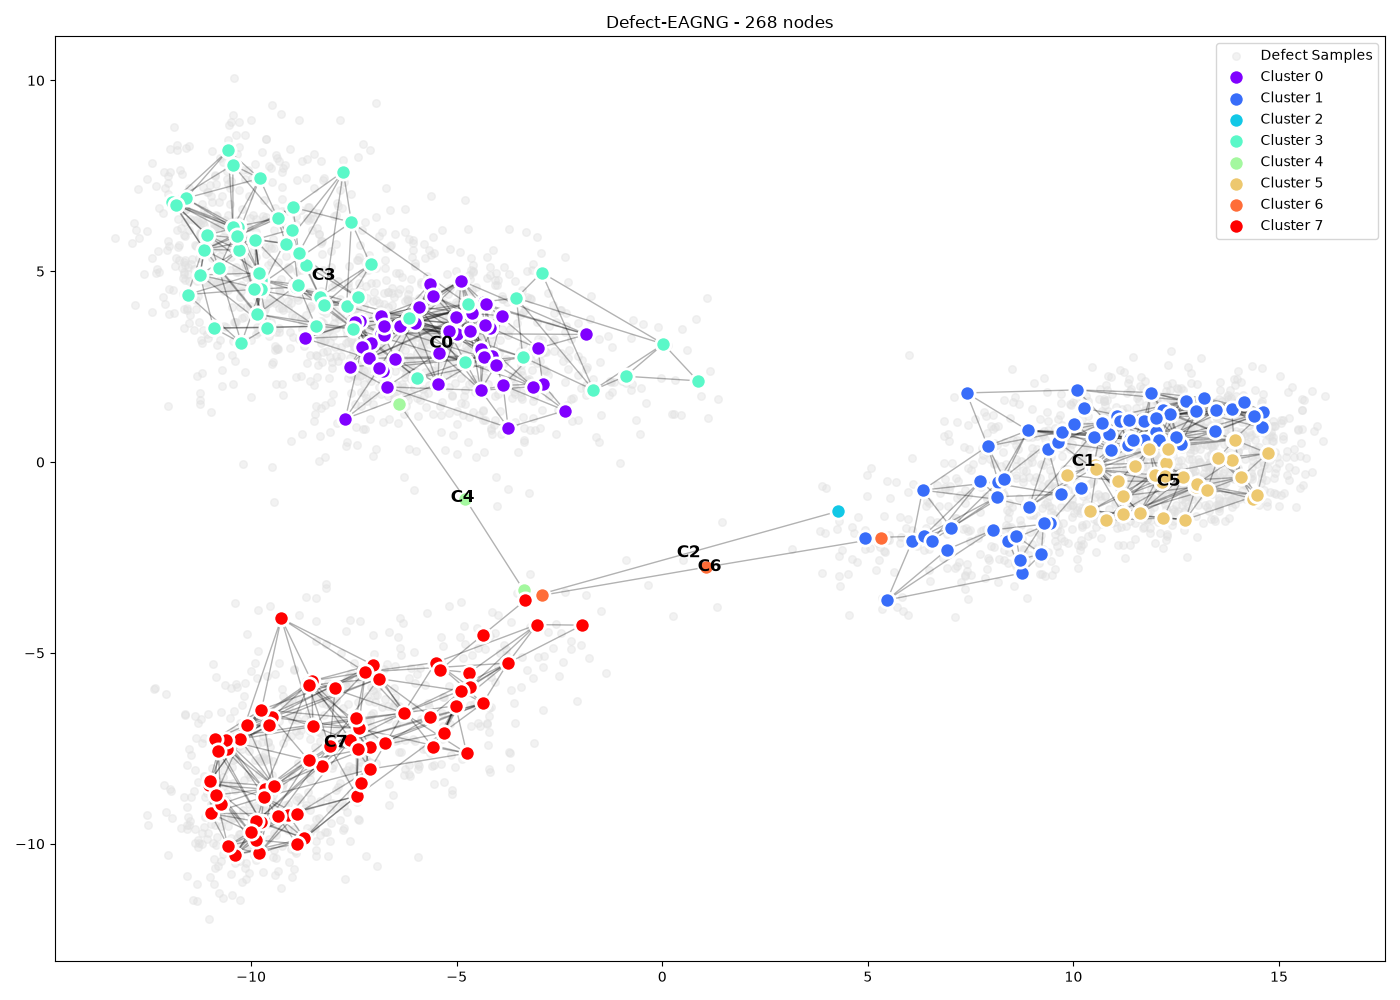
\includegraphics[width=0.85\linewidth]{figures/c4/c4_eagng.png}
    \caption{Trực quan hóa cấu trúc mạng và phân cụm của thuật toán EAGNG tại bước $3000$.}
    \caption*{Ghi chú: Mô hình xây dựng thành công $268$ nút với $8$ cụm phân biệt rõ ràng từ C0 đến C7.}
    \label{fig:vis_eagng}
\end{figure}

Cấu trúc mạng do EAGNG tạo ra thể hiện sự tương thích cao với phân bố tự nhiên của dữ liệu lỗi. Như được thể hiện trong Hình~\ref{fig:vis_eagng}, EAGNG tự động hình thành $268$ nút và tách biệt chính xác $8$ cụm lỗi riêng biệt từ C0 đến C7 mà không cần khai báo trước số lượng cụm. Các cạnh liên kết giữa các nút phản ánh đúng mật độ liên tục của dữ liệu trong từng vùng không gian, trong khi ranh giới giữa các cụm được phân định rõ ràng nhờ cơ chế loại bỏ cạnh lỗi thời.

\begin{figure}[htbp]
    \centering
    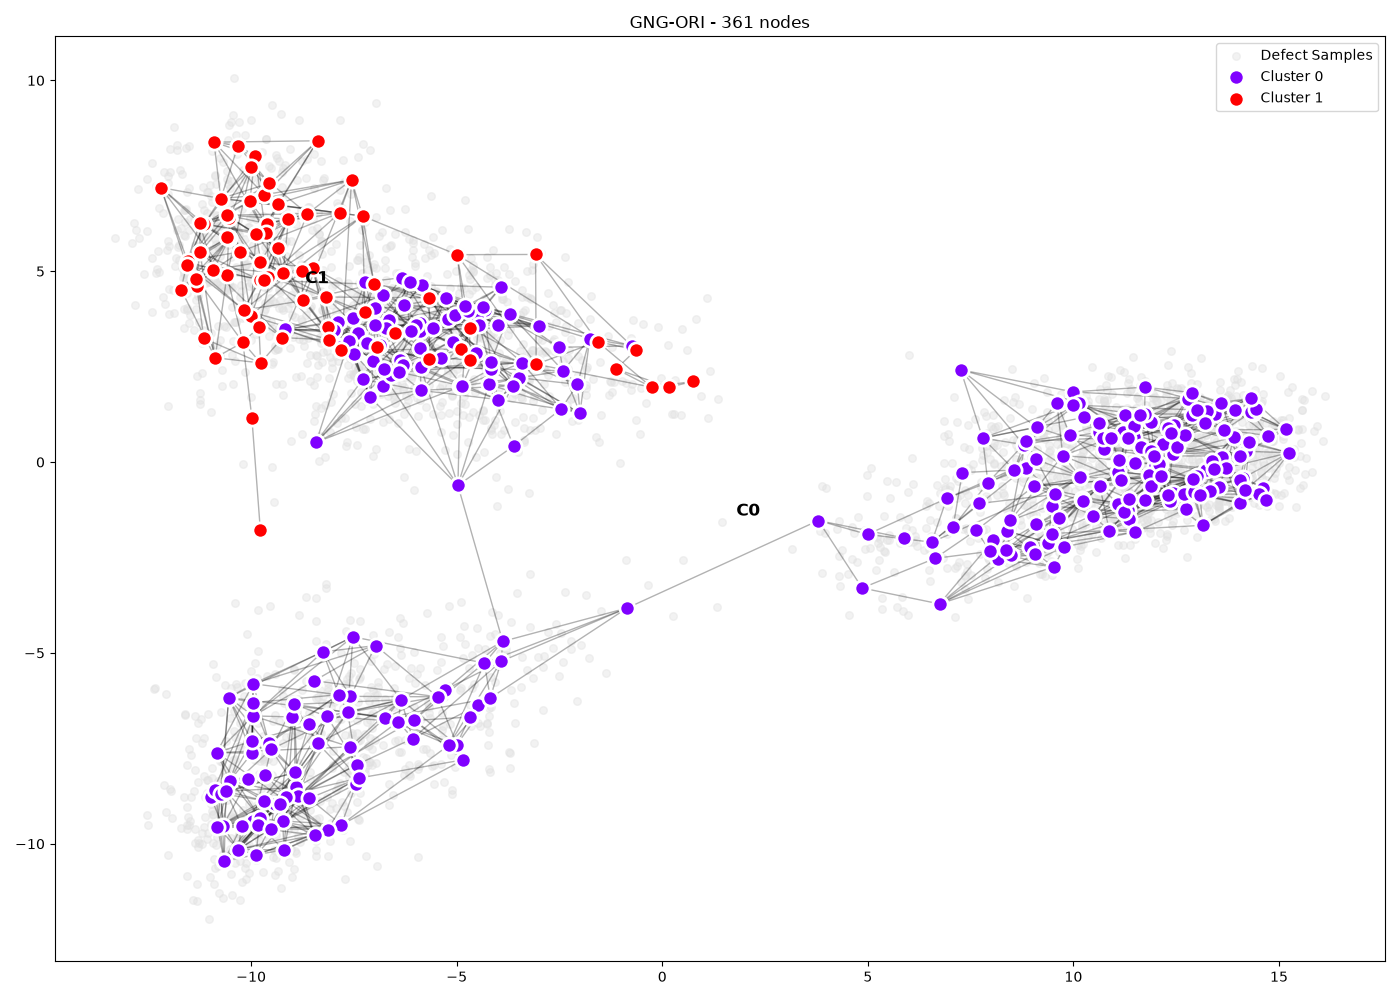
\includegraphics[width=0.85\linewidth]{figures/c4/c4_gng.png}
    \caption{Trực quan hóa cấu trúc mạng của thuật toán GNG truyền thống tại bước $3000$.}
    \caption*{Ghi chú: Mạng phát triển lên $361$ nút nhưng bị gộp thành $2$ cụm lớn không chính xác.}
    \label{fig:vis_gng}
\end{figure}

Ngược lại, cấu trúc của GNG truyền thống bị suy thoái nghiêm trọng dưới tác động của dịch chuyển khái niệm. Như mô tả ở Hình~\ref{fig:vis_gng}, GNG truyền thống khởi tạo tới $361$ nút nhưng chỉ phân tách được $2$ cụm lớn C0 và C1. Các nút mạng nối liền các vùng dữ liệu vốn dĩ thuộc các dạng lỗi khác nhau, dẫn đến hiện tượng trộn lẫn các lớp lỗi và làm giảm chỉ số ARI xuống $21{,}0\%$.

\begin{figure}[htbp]
    \centering
    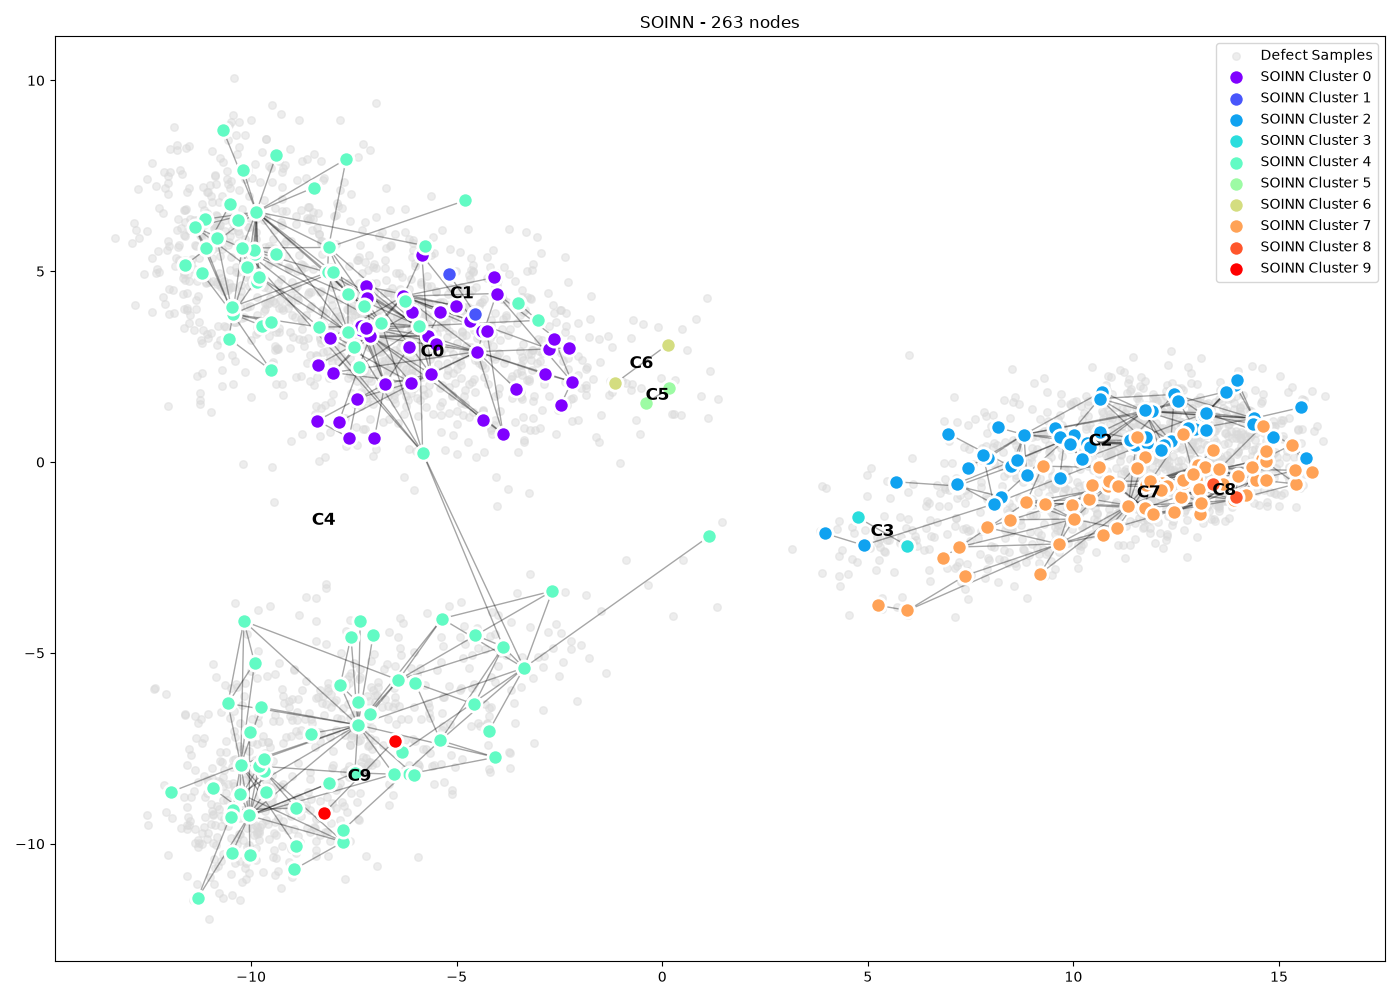
\includegraphics[width=0.85\linewidth]{figures/c4/c4_soinn.png}
    \caption{Trực quan hóa cấu trúc mạng của thuật toán SOINN tại bước $3000$.}
    \caption*{Ghi chú: Mạng khởi tạo $263$ nút nhưng bị phân mảnh thành $10$ cụm do ngưỡng phân tách quá khắt khe.}
    \label{fig:vis_soinn}
\end{figure}

Đối với thuật toán SOINN, mạng gặp phải hiện tượng phân mảnh cụm quá mức. Như thể hiện trong Hình~\ref{fig:vis_soinn}, SOINN tạo ra $263$ nút và chia dữ liệu thành $10$ cụm riêng biệt từ C0 đến C9. Một số cụm nhỏ lẻ bị cô lập hoàn toàn dù thuộc cùng một dạng phân bố lỗi gốc, làm giảm hiệu quả tổng hợp thông tin cho các công đoạn phân loại tự động phía sau.

\subsection{Tổng hợp kết quả so sánh định lượng}
\label{sec:4_2_5_summary}

Bảng~\ref{tab:metrics_summary} tổng hợp các chỉ số đánh giá hiệu năng của phương pháp đề xuất EAGNG so với các phương pháp cơ sở tại thời điểm kết thúc chuỗi thực nghiệm ($3000$ mẫu). Các chỉ số bao gồm chỉ số Rand điều chỉnh (ARI), chỉ số thông tin tương hỗ chuẩn hóa (NMI), độ thuần khiết, số lượng nút mạng, và tổng thời gian tính toán tích lũy. Ngoài ra, kết quả của thuật toán Oracle K-Means \cite{macqueen1967methods} được đưa vào để làm chuẩn mực so sánh, mặc dù phương pháp này yêu cầu gán nhãn trước và không thể áp dụng trực tiếp trong môi trường học trực tuyến. Chính vì vậy, các chỉ số của Oracle K-Means khi biết trước số cụm được xem như giới hạn trên về hiệu năng phân cụm mà các thuật toán học trực tuyến có thể hướng tới.

\begin{table}[htbp]
    \centering
    \caption{Bảng tổng hợp chỉ số hiệu năng định lượng tại thời điểm mẫu thứ $3000$.}
    \label{tab:metrics_summary}
    \begin{tabular}{|l|c|c|c|c|c|}
        \hline
        Phương pháp & ARI & NMI & Độ thuần khiết & Số nút & Thời gian (giây) \\
        \hline
        EAGNG (Đề xuất) & 89,5\% & 92,7\% & 95,2\% & 268 & 16,39 \\
        SOINN \cite{furao2006soinn} & 76,3\% & 87,4\% & 80,8\% & 263 & 6,30 \\
        GNG \cite{fritzke1995growing} & 21,0\% & 47,4\% & 40,0\% & 361 & 23,69 \\
        Oracle K-Means \cite{macqueen1967methods} & 97,9\% & 97,5\% & 99,2\% & - & - \\
        \hline
    \end{tabular}
\end{table}

Các số liệu trong Bảng~\ref{tab:metrics_summary} khẳng định rằng EAGNG đạt sự cân bằng tối ưu giữa chất lượng phân cụm và chi phí tài nguyên tính toán. Thuật toán EAGNG vượt trội hơn SOINN $13{,}2$ điểm phần trăm về chỉ số ARI và $14{,}4$ điểm phần trăm về độ thuần khiết, trong khi tiết kiệm được $30{,}8\%$ thời gian tính toán và giảm $25{,}8\%$ số lượng nút so với GNG truyền thống.
\section{Thảo luận Kết quả và Đóng góp của Nghiên cứu}
\label{sec:4_3_discussion_contributions}

Mục này tiến hành thảo luận sâu về cơ chế hoạt động hợp nhất của thuật toán EAGNG, đồng thời phân tích những đóng góp về mặt khoa học và giá trị ứng dụng thực tiễn trong bài toán kiểm tra chất lượng màn hình điện thoại. Các luận điểm được xây dựng dựa trên sự tổng hợp chuỗi kết quả thực nghiệm đã trình bày tại Mục \ref{sec:4_2_results}.

\subsection{Thảo luận về hiệu năng hệ thống và tính hợp nhất cấu trúc}
\label{sec:4_3_1_system_performance}

Mô hình EAGNG thể hiện sự vượt trội về mặt tổng thể nhờ sự phối hợp đồng bộ giữa bộ đệm tích lũy bằng chứng và cơ chế tự điều chỉnh độ linh hoạt cấu trúc. Sự kết hợp này giúp thuật toán duy trì chỉ số điều chỉnh Rand ở mức $0{,}895$ và chỉ số thông tin tương hỗ chuẩn hóa ở mức $0{,}927$ tại thời điểm xử lý mẫu thứ $3000$. Các kết quả thực nghiệm thu được từ Hình \ref{fig:drift_ari} và Hình \ref{fig:drift_nmi} ở Mục \ref{sec:4_2_1_concept_drift} cho thấy mô hình không bị suy giảm hiệu năng khi gặp dịch chuyển khái niệm liên tục. Ngoài ra, chỉ số dịch chuyển trọng số của các nút cũ duy trì dưới mức $0{,}5$ trong Hình \ref{fig:topo_stability} chứng minh hiện tượng quên thảm họa đã được kiểm soát hiệu quả.

Mặc dù nghiên cứu chưa thực hiện các bài kiểm tra bóc tách riêng biệt từng thành phần cải tiến, sự tương tác đồng thời giữa bộ đệm và quy tắc cập nhật trọng số vẫn được minh chứng rõ ràng thông qua hành vi tổng thể của mô hình. Bộ đệm đóng vai trò lưu giữ các mẫu dữ liệu tạm thời, ngăn chặn việc tạo nút hoặc xóa cạnh quá sớm khi phân bố dữ liệu biến đổi đột ngột. Đồng thời, cơ chế tự thích ứng điều chỉnh tốc độ học của các nút mới lên mức $8{,}9$ trong Hình \ref{fig:topo_stability}, đảm bảo khả năng tiếp thu tri thức mới mà không làm suy biến cấu trúc không gian đã tích lũy. Việc đánh giá mô hình dưới dạng một hệ thống hợp nhất phản ánh chính xác trạng thái hoạt động thực tế trong dây chuyền công nghiệp, nơi các thành phần thuật toán phải phối hợp liên tục theo thời gian thực.

\subsection{Đóng góp khoa học và ý nghĩa ứng dụng thực tiễn}
\label{sec:4_3_2_contributions}

Về mặt lý thuyết và khoa học, nghiên cứu đóng góp một phương pháp học trực tuyến không giám sát có khả năng tự điều chỉnh cấu trúc mạng theo sự tiến hóa của luồng dữ liệu. Đóng góp của phương pháp EAGNG thể hiện qua ba khía cạnh chính bao gồm: (i) đề xuất cơ chế tích lũy bằng chứng dựa trên bộ đệm để giảm thiểu tác động của nhiễu cục bộ trong chuỗi dữ liệu theo thời gian, (ii) xây dựng chỉ số đo lường sự cân bằng giữa tính linh hoạt và tính ổn định dựa trên độ dịch chuyển chuẩn L2 của trọng số nơ-ron, và (iii) tối ưu hóa mật độ nút mạng giúp duy trì chi phí tính toán ổn định theo chuỗi thời gian xử lý. Phương pháp này mở ra hướng đi cho việc ứng dụng thuật toán học tăng trưởng \cite{fritzke1995growing, furao2006soinn} trong các bài toán phân loại không giám sát trên luồng dữ liệu công nghiệp.

Về mặt ứng dụng thực tiễn, mô hình EAGNG cung cấp một giải pháp tự động hóa khả thi cho hệ thống kiểm tra và phân loại lỗi màn hình điện thoại trong sản xuất. Với thời gian nhịp xử lý trung bình đạt $5{,}46$ mili-giây trên mỗi mẫu như thể hiện trong Hình \ref{fig:takt_time}, mô hình hoàn toàn đáp ứng các tiêu chuẩn khắt khe về tốc độ xử lý của dây chuyền tự động. Việc tự động hình thành $8$ cụm lỗi riêng biệt từ C0 đến C7 trong Hình \ref{fig:vis_eagng} giúp giảm thiểu sự phụ thuộc vào quá trình gán nhãn thủ công. Kết quả này hỗ trợ các kỹ sư nhà máy nhanh chóng phát hiện các dạng lỗi mới xuất hiện, góp phần nâng cao tỷ lệ thành phẩm và giảm chi phí vận hành dây chuyền.
%\section{Mô phỏng giao diện kiểm tra khuyết tật màn hình thời gian thực}
Giao diện ứng dụng mô phỏng kiểm tra khuyết tật màn hình thời gian thực được phát triển nhằm trực quan hóa các chỉ số vận hành và cấu trúc mạng tự điều chỉnh của mô hình EAGNG trong quá trình xử lý dòng dữ liệu. Hệ thống giao diện tích hợp trực tiếp luồng xử lý ảnh với mạng nơ-ron học trực tuyến, giúp giám sát các tham số phân cụm và thời gian đáp ứng của mô hình ở từng bước thời gian. Cấu trúc giao diện được chia thành các khu vực chức năng chính bao gồm (i) khung hiển thị ảnh kiểm tra và kết quả nhận dạng, (ii) khung biểu diễn đồ thị cấu trúc topology của mạng EAGNG, (iii) khung đo lường các chỉ số hiệu năng phân cụm thời gian thực, và (iv) khung quản lý tiến trình thực nghiệm đối sánh. Việc phân chia cấu trúc này bảo đảm tính minh bạch trong quá trình theo dõi sự biến đổi cấu trúc mạng khi xuất hiện hiện tượng trôi dạt khái niệm trên dòng dữ liệu.

Khung hiển thị hình ảnh kiểm tra nằm ở góc trên bên trái thể hiện trực tiếp mẫu ảnh đang được nạp vào hệ thống cùng thông tin phân loại chi tiết. Trong Hình \ref{fig:c4_app_demo}, mẫu ảnh thứ 1246 trên tổng số 3000 mẫu đại diện cho khuyết tật dạng hình tam giác được đưa vào xử lý và thu được kết quả nhận dạng chính xác. Ngay bên cạnh, khung biểu diễn đồ thị mạng EAGNG trực quan hóa sự phân bố không gian của 268 nút mạng cùng 51 liên kết cạnh giữa các nút. Đồ thị cấu trúc phản ánh sự hình thành của các cụm dữ liệu phân biệt từ C0 đến C7, trong đó số lượng cụm hoạt động duy trì ở mức bốn cụm chính tương ứng với các phân bố đặc trưng đã tích lũy. Việc hiển thị trực quan đồ thị topology giúp quan sát sự dịch chuyển của các nút mạng và phản ứng thích ứng cấu trúc khi mẫu dữ liệu mới thuộc lớp tam giác xuất hiện.

\begin{figure}[htbp]
\centering
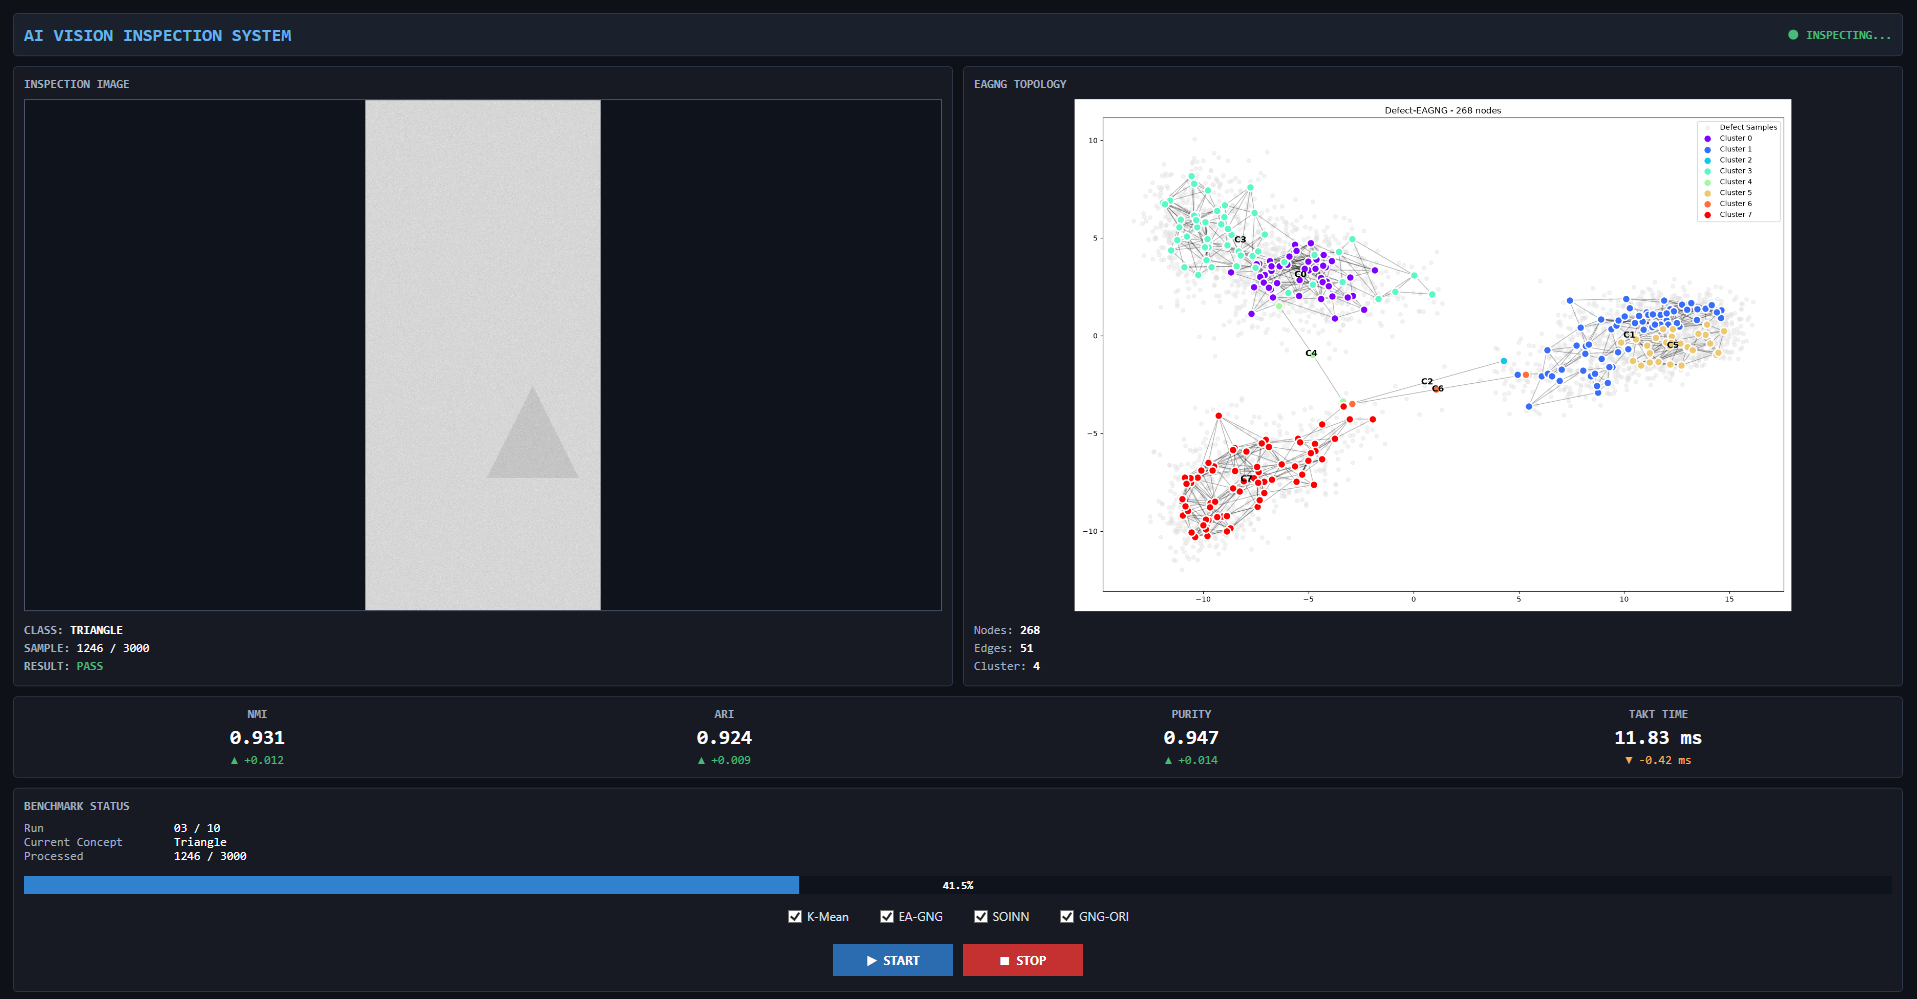
\includegraphics[width=0.98\textwidth]{figures/c4/c4_AppDemo.png}
\caption{Giao diện ứng dụng mô phỏng kiểm tra khuyết tật màn hình thời gian thực trên mạng EAGNG.}
\label{fig:c4_app_demo}
\end{figure}

Khung đo lường chỉ số thời gian thực và quản lý tiến trình thực nghiệm nằm ở phía dưới cung cấp các thông số định lượng cập nhật theo từng mẫu dữ liệu. Kết quả ghi nhận tại thời điểm xử lý mẫu thứ 1246 đạt chỉ số NMI là 0,931, chỉ số ARI đạt 0,924 và độ tinh khiết Purity đạt 0,947. Thời gian nhịp sản xuất Takt Time duy trì ở mức 11,83 millisecond trên một mẫu, khẳng định khả năng đáp ứng yêu cầu vận hành thời gian thực trên dây chuyền công nghiệp. Khung quản lý tiến trình ở đáy giao diện ghi nhận lượt chạy thứ ba trên tổng số mười lượt thực nghiệm với tiến độ hoàn thành đạt 41,5 phần trăm cho kịch bản trôi dạt khái niệm dạng hình tam giác. Hệ thống cho phép kích hoạt đồng thời các thuật toán đối sánh bao gồm K-Means, EAGNG, SOINN và GNG-ORI để so sánh hiệu năng trực tiếp dưới cùng một điều kiện dòng dữ liệu đầu vào \cite{fritzke1995growing, furao2006soinn}.

Mô hình giao diện vận hành ổn định và không xảy ra hiện tượng tắc nghẽn dữ liệu trong suốt chuỗi kiểm thử 3000 mẫu. Tần số cập nhật giao diện được tối ưu hóa thông qua cơ chế bất đồng bộ giữa luồng tính toán mô hình và luồng hiển thị đồ họa. Mức tiêu tốn tài nguyên hệ thống duy trì ở ngưỡng an toàn, đáp ứng tiêu chuẩn triển khai thực tế trên các thiết bị máy tính công nghiệp. Sự suy giảm thời gian nhịp sản xuất xuống mức 11,83 millisecond minh chứng cho hiệu quả của cơ chế hoãn chèn nút và rào chắn mật độ cục bộ trong việc tối ưu hóa chi phí tính toán khoảng cách Euclid.


\section*{Kết luận Chương 4}
\addcontentsline{toc}{section}{Kết luận Chương 4}


Chương \ref{chap:c4} đã trình bày chi tiết các kết quả thực nghiệm từ việc xây dựng dữ liệu giả lập, huấn luyện mô hình trích xuất đặc trưng đến việc triển khai hệ thống học liên tục trên phần mềm demo thực tế. Dựa trên các số liệu định lượng và phân tích trực quan, có thể rút ra các kết luận quan trọng sau:

\begin{itemize}
    \item \textbf{Về dữ liệu và tiền xử lý:} Thuật toán sinh dữ liệu giả lập đã tạo ra nguồn dữ liệu huấn luyện phong phú, khắc phục được tình trạng thiếu hụt mẫu lỗi trong công nghiệp. Đặc biệt, việc tích hợp kênh Entropy cục bộ đã chứng minh được vai trò quyết định trong việc nâng cao khả năng phát hiện các lỗi có độ tương phản thấp (như đường kẻ mờ), cải thiện đáng kể độ nhạy của mô hình so với phương pháp chỉ sử dụng ảnh mức xám truyền thống.
    
    \item \textbf{Về khả năng học liên tục:} Mạng Growing Neural Gas (GNG) đã giải quyết thành công bài toán thích nghi cấu trúc. Thông qua các cơ chế sinh nơ-ron (Insertion) và loại bỏ liên kết (Edge Removal), hệ thống đã học được các tác vụ mới (lỗi hình chữ nhật, lỗi tam giác) mà không làm suy giảm độ chính xác trên các tác vụ cũ (lỗi đốm tròn, lỗi đường kẻ). Kết quả so sánh cho thấy GNG duy trì độ chính xác trung bình trên 96\% qua 3 giai đoạn, vượt trội hoàn toàn so với phương pháp tinh chỉnh (Fine-tuning) vốn bị ảnh hưởng nặng nề bởi hiện tượng quên thảm họa.
    
    \item \textbf{Về tính khả thi ứng dụng:} Trong quá trình benchmark trên 3.000 ảnh, thuật toán EAGNG hoàn thành toàn bộ quá trình xử lý trong khoảng 16.39 giây, tương ứng với takt time trung bình khoảng 5.46 ms/ảnh. Ở 50 ảnh cuối của tập benchmark, takt time đạt khoảng 10.19 ms/ảnh (takt time tăng lên do cần xử lý thêm các dữ liệu có trong bộ đệm). Kết quả cho thấy hệ thống có khả năng đáp ứng yêu cầu xử lý trực tuyến với tốc độ cao trong môi trường kiểm tra sản xuất.
\end{itemize}

Những kết quả khả quan này là minh chứng thực tiễn cho tính đúng đắn của phương pháp luận đã đề ra. Trên cơ sở đó, phần Kết Luận sẽ tổng kết lại toàn bộ nội dung luận văn, đồng thời chỉ ra những hạn chế còn tồn tại và đề xuất các hướng phát triển tiềm năng để hoàn thiện hệ thống trong tương lai.